% !TEX root = ../notes_template.tex
\chapter{Linear Transformations}\label{chp:lintrans}

% \minitoc

% Inset a quote for the chapter
\begin{flushright}
\textit{``Though a bit of an exaggeration, it can be said that a mathematical problem can be solved only if it can be reduced to a calculation in linear algebra. And a calculation in linear algebra will reduce ultimately to the solving of a system of linear equations, which in turn comes down to the manipulation of matrices.''}\\
% Draw a small line at the end of the quote
\rule{0.5\textwidth}{.4pt}\\
\textbf{Thomas A Garrity} \small{in \textit{All the Mathematics You Missed.}}
\end{flushright}

I concede that the first two chapters were a bit dry. Hopefully, you will find topics from now on a bit more interesting. Linear algebra is the study of linear transformations. We already saw an example of a linear transformation in Section~\ref{sec:ch01-lin-func}. We will look at linear transformations in in their general form and see how matrices can be used to represent and understand them.

\section{What is a linear transformation?}\label{sec:ch03-lin-trans-def}
A \textit{linear transformation} or \textit{linear map} $T$ is a function between two vector spaces that satisfies the homgeneity (scaling) and additivity properties. In this course, we will particularly be interested in linear transformation from $\mb{R}^m$ to $\mb{R}^n$, i.e. $T: \mb{R}^m \to \mb{R}^n$. These satisfy the following two properties:
\begin{enumerate}
    \item \textbf{Additivity:} For all $\mf{x}, \mf{y} \in \mb{R}^m$, $T(\mf{x} + \mf{y}) = T(\mf{x}) + T(\mf{y})$.
    \item \textbf{Homogeneity:} For all $\mf{x} \in \mb{R}^m$ and $c \in \mb{R}$, $T(c\mf{x}) = cT(\mf{x})$.
\end{enumerate}
Note that linearity property allow us to move the transformation operation into the paranthesis for the addition or scalar multiplication of the arguments. The above properties also imply the following:
\begin{itemize}
    \item \textbf{Superposition:} For all $\mf{x}, \mf{y} \in \mb{R}^m$ and $c, d \in \mb{R}$, $T\pp{c\mf{x} + d\mf{y}} = T\pp{c\mf{x}} + T\pp{d\mf{y}} = cT\pp{\mf{x}} + dT\pp{\mf{y}}$.
    
    Linear combination of two vectors $\mf{x}_1, \mf{x}_2 \in \mb{R}^m$  in the transformations arugment results in the same linear combination of the individual transformed vectors $T\pp{\mf{x}_1}, T\pp{\mf{x}_2} \in \mb{R}^n$. 
    
    \item \textbf{Zero input:} $T(\mf{0}_m) = \mf{0}_n$, where $\mf{0}_m \in \mb{R}^m$ and $\mf{0}_n \in \mb{R}^n$.
    
    The zero vector from $\mb{R}^m$ maps to the zero vector from $\mb{R}^m$ under any linear transformation.
\end{itemize}

The linear functions we considered in Section~\ref{sec:ch01-lin-func} are special cases of linear transformations, where $n = 1$. We will now look at some examples of transformations that are linear and some that are not.

\begin{boxedstuff}
\begin{example}
Consider the transformation $T: \mb{R}^2 \to \mb{R}^2$ defined by $T\pp{\bmx x_1 \\ x_2 \emx} = \bmx 2x_1 \\ 3x_2 \emx$. This transformation is linear because it satisfies the properties of additivity and homogeneity. For example, $T\pp{\alpha \bmx x_1 \\ x_2 \emx + \beta \bmx y_1 \\ y_2 \emx} = T\pp{\bmx \alpha x_1 + \beta y_1 \\ \alpha x_2 + \beta y_2 \emx} = \bmx 2\pp{\alpha x_1 + \beta y_1} \\ 3\pp{\alpha x_2 + \beta y_2} \emx = \alpha \bmx 2x_1 \\ 3x_2 \emx + \beta \bmx 2y_1 \\ 3y_2 \emx = \alpha T\pp{\bmx x_1 \\ x_2 \emx} + \beta T\pp{ \bmx y_1 \\ y_2 \emx}$.
\end{example}

\begin{example}
Consider the transformation $T: \mb{R}^2 \to \mb{R}^2$ defined by $T\pp{\bmx x_1 \\ y \emx} = \bmx x^2 \\ y^2 \emx$. This transformation is not linear because it does not satisfy the property of homogeneity. For example, $T\pp{2\bmx 1 \\ 2 \emx} = T\pp{\bmx 2 \\ 4 \emx} = \bmx 4 \\ 16 \emx \neq 2\bmx 1 \\ 4 \emx = 2T\pp{\bmx 1 \\ 2 \emx}$.
\end{example}
\end{boxedstuff}

Now you can try your hand at the following exercises. Note that to show $T: \mb{R}^m \to \mb{R}^n$ is not a linear transformation, you only need to show an example that does not satisfy additivity and homogeneity. However, to show that a transformation is linear, you need to demonstrate that $T$ satisfies both properties for all possible vectors in $\mb{R}^m$. The proof of linearity can be a bit more involved than showing non-linearity.
\begin{boxedstuff}
\begin{problem}
Which of the following transformations are linear?
\begin{enumerate}
    \item $T: \mb{R}^2 \to \mb{R}^2$, $T\pp{\bmx x_1 \\ x_2 \emx} = \bmx x_1 + x_2 \\ x_1 - x_2 \emx$
    \item $T: \mb{R}^2 \to \mb{R}^3$, $T\pp{\bmx x_1 \\ x_2 \emx} = \bmxc x_1 + 1 \\ x_2 + 2 \\ 3x_1 + 2x_2 - 1\emx$
    \item $T: \mb{R}^3 \to \mb{R}^2$, $T\pp{\bmx x_1 \\ x_2 \\ x_3\emx} = \bmx 0 \\ 0 \emx$
\end{enumerate}
\end{problem}
\end{boxedstuff}

\section{Matrices represent linear transformations}\label{sec:ch03-mat-lin-trans}
In Section~\ref{sec:ch01-lin-func}, we saw that any linear function $f: \mb{R}^m \to \mb{R}$ can be represented by a fixed $\mf{w} \in \mb{R}^m$, and $f\pp{\mf{x}} = \mf{w}^\top\mf{x}$. We can extend this idea to linear transformations from $\mb{R}^m$ to $\mb{R}^n$. Any linear transformation $T: \mb{R}^m \to \mb{R}^n$ can be represented by a fixed $n \times m$ matrix $\mf{A} \in \mb{R}^{n \times m}$, such that $T\pp{\mf{x}} = \mf{A}\mf{x}$; $\mf{A}$ is the \textit{matrix representation} of the linear transformation $T$.
\begin{equation}
    \begin{split}
        \mf{y} = T\pp{\mf{x}} = \mf{A}\mf{x} &= \bmxc a_{11} & a_{12} & \cdots & a_{1m}\\ a_{21} & a_{22} & \cdots & a_{2m}\\ \vdots & \vdots & \ddots & \vdots\\ a_{n1} & a_{n2} & \cdots & a_{nm} \emx \bmxc x_1 \\ x_2 \\ \vdots \\ x_m\emx \\
        \bmxc y_1 \\ y_2 \\ \vdots \\ y_n \emx &= \bmxc a_{11}x_1 + a_{12}x_2 + \cdots + a_{1m}x_m \\ 
        a_{21}x_1 + a_{22}x_2 + \cdots + a_{2m}x_m \\
        \vdots \\
        a_{n1}x_1 + a_{n2}x_2 + \cdots + a_{nm}x_m\emx 
    \end{split}
    \label{eq:ch03-lin-trans-mat-rep}
\end{equation}
This shows that all linear transformation are essentially a set of simultaneous linear equations, where $y_i = a_{i1}x_1 + a_{i2}x_2 + \cdots + a_{im}x_m$, $1 \leq i \leq n$.

Let's assume that I give you a Python/Julia function, which takes in vectors from $\mb{R}^m$, does some computation, and returns vectors from $\mb{R}^n$. I also tell to you that this function is linear. You do not want to use this function. If you knew the matrix $\mf{A}$ corresponding to this linear transformation, then you can compute the function yourself. But, how can you find the matrix corresponding this function? Remember how how we identified the entries of $\mf{w} \in \mb{R}^m$ (Section~\ref{sec:ch01-lin-func}) in the case of linear functions? We had used the unit vectors of $\mb{R}^m$ to get  the $w_i$s. Turns out, we do the exact same thing, and the elements of $\mf{A}$ will be revealed to us by the output of the linear transformation to the $m$ unit vectors of $\mb{R}^m$. If $\mf{a}_i$ is the $i^{th}$ column of $\mf{A}$, then 
$\mf{a}_i = T\pp{\mf{e}_i}, \,\, \mf{e}_i \in \mb{R}^m$. \textcolor{red}{Can you explain why?}

% \begin{boxedstuff}
%     \begin{problem}
%         Consider the linear transformation $T: \mb{R}^m \to \mb{R}^n$,  with the corresponding matrix $\mf{A} = \bmx T\pp{\mf{e}_1} & T\pp{\mf{e}_2} & \cdots & T\pp{\mf{e}_m}\emx \in \mb{R}^{n \times m}$. Unfortunately, all you have is the following set $\lc \rc$ 
%     \end{problem}
% \end{boxedstuff}

\section{Matrix multiplication and linear transformations}\label{sec:ch03-mat-mult-lin-trans}
Consider the following two transformations $T_A$ and $T_B$: 
\[ \begin{split}
    \mf{y} & = \bmx y_1 \\ y_2 \emx = T_A\pp{\mf{x}} = \mf{A}\mf{x} = \bmx a_{11} & a_{12} \\ a_{21} & a_{22}\emx \bmx x_1 \\ x_2 \emx = \bmx a_{11}x_1 + a_{12}x_2 \\ a_{21}x_1 + a_{22}x_2 \emx\\
    \mf{v} &= \bmx v_1 \\ v_2 \emx = T_B\pp{\mf{u}} = \mf{B}\mf{u} = \bmx b_{11} & b_{12} \\ b_{21} & b_{22}\emx \bmx u_1 \\ u_2 \emx = \bmx b_{11}u_1 + b_{12}u_2 \\ b_{21}u_1 + b_{22}u_2 \emx
\end{split}
\]
Let $\mf{u} \in \mb{R}^2$ and $\mf{v} = T_C\pp{\mf{u}} = T_A \circ T_B\pp{\mf{u}} = T_A\pp{T_B\pp{\mf{u}}}$. We can write this as:
\[ \mf{v} = T_C\pp{\mf{u}} = T_A\pp{T_B\pp{\mf{u}}} = T_A\pp{\mf{B}\mf{u}} = \mf{A}\mf{B}\mf{u} \]
This implies that the matrix $\mf{A}\mf{B}$ corresponds to the transformation $T_C$. This is an important result. Matrix multiplication can be seen as the process of composing two linear transformations, i.e. applying two linear transoformation one after the other on a vector $\mf{x}$ (from right to left).
\[ \begin{split}
    \mf{v} = \bmx v_1 \\ v_2 \emx &= T_A\pp{T_B\pp{\mf{u}}} = T_A\pp{\bmx b_{11}u_1 + b_{21}u_2 \\ b_{21}u_1 + b_{22}u_2 \emx} = \bmx a_{11}b_{11}u_1 + a_{11}b_{21}u_2 + a_{12}b_{21}u_1 + a_{12}b_{22}u_2 \\ a_{21}b_{11}u_1 + a_{21}b_{21}u_2 + a_{22}b_{21}u_1 + a_{22}b_{22}u_2 \emx \\
    &= \bmx \pp{a_{11}b_{11} + a_{12}b_{21}}u_1 + \pp{a_{11}b_{21} + a_{12}b_{22}}u_2 \\ \pp{a_{21}b_{11} + a_{22}b_{21}}u_1 + \pp{a_{21}b_{21} + a_{22}b_{22}}u_2 \emx = \bmx a_{11}b_{11} + a_{12}b_{21} + a_{11}b_{21} + a_{12}b_{22} \\ a_{21}b_{11} + a_{22}b_{21} + a_{21}b_{21} + a_{22}b_{22} \emx \bmx u_1 \\ u_2 \emx
\end{split} \]
The above equation shows how the strange definition of matrix multiplication comes out beautifully from the composition of linear transformations. Although, we have taken a simple example of $2 \times 2$ matrices, the idea extends to matrices of any size, as long as the dimensions are compatible for multiplication.

\begin{boxedstuff}
    \begin{problem}
        Consider the matrix multiplication, $\mf{C} = \mf{A}\mf{B}$ with $\mf{A} \in \mb{R}^{n \times p}$ and $\mf{B} \in \mb{R}^{p \times m}$. We know that this operation can be seen as the composition of two linear transformations. Using the idea of composition of linear transformations, show that the the $i^{th}$ column of the matrix $\mf{C}$ is given by the linear combination of the columns of $\mf{A}$ with the coefficients from the $i^{th}$ column of $\mf{B}$.
    \end{problem}
\end{boxedstuff}

\section{System of linear equations}\label{sec:ch03-sys-lin-eqn}
An important use of matrices and linear transformations is in solving systems of linear equations. Consider the following system of linear equations which we have seen from our high school years,
\begin{equation}
    \begin{split}
        a_{11}x_1 + a_{12}x_2 + &\cdots + a_{1m}x_m = b_1\\
        a_{21}x_1 + a_{22}x_2 + &\cdots + a_{2m}x_m = b_2\\
        &\vdots\\
        a_{n1}x_1 + a_{n2}x_2 + &\cdots + a_{nm}x_m = b_n
    \end{split}
    \label{eq:ch03-sys-lin-eqn}
\end{equation}
Here, the coefficients $a_{ij}$ and $b_{i}$ are known, and we are interested in solving for the unknowns $x_{j}$. We know how to solve these equations and also know the geometric associated with these equations. Each row represents a hyperplane in $\mb{R}^m$ and the solution, if it exists, is the set of all points in the intersection of the $n$ planes in $\mb{R}^m$.

We can write the above system of linear equations in the matrix form as the following,
\begin{equation}
    \begin{split}
        a_{11}x_1 + \cdots& + a_{1m}x_m = b_1\\
        &\vdots\\
        a_{n1}x_1 + \cdots& + a_{nm}x_m = b_n
    \end{split} \longrightarrow \mf{A}\mf{x} = \mf{b}, \quad \mf{A \in \mb{R}^{n \times m}}, \mf{x} \in \mb{R}^m, \mf{b} \in \mb{R}^n
\end{equation}

\subsection{Geometry interpretation of linear equations}
The matrix representation offers a new geometrical view of the system of linear equations in Eq~\ref{eq:ch03-sys-lin-eqn}. The above geometrical interpreation of viewing each equation as a hyperplane in $\mb{R}^m$ is referred to as the \textit{row view}. The other geomtric view is the \textit{column view}, which can be easily seen from the following way of writing Eq.~\ref{eq:ch03-sys-lin-eqn}.
\begin{equation}
    \mf{A}\mf{x} = \mf{b} \longrightarrow x_1\mf{a}_1 + x_2\mf{a}_2 + \cdots + x_m \mf{a}_m = \mf{b}
\end{equation}
The vector $\mf{b}$ is a linear combination of the columns of $\mf{A}$, where the $m$ columns $\mf{a}_i$ and $\mf{b}$ are know, and the unknows $x_i$ are the mixture of the linear combination that we are interested in determining. The row and column view of a system of two linear equations with two unknowns are depicted in Figure~\ref{fig:ch03-lineq-row-view} and Figure~\ref{fig:ch03-lineq-col-view}, respectively.

\begin{figure}[h]
    \centering
    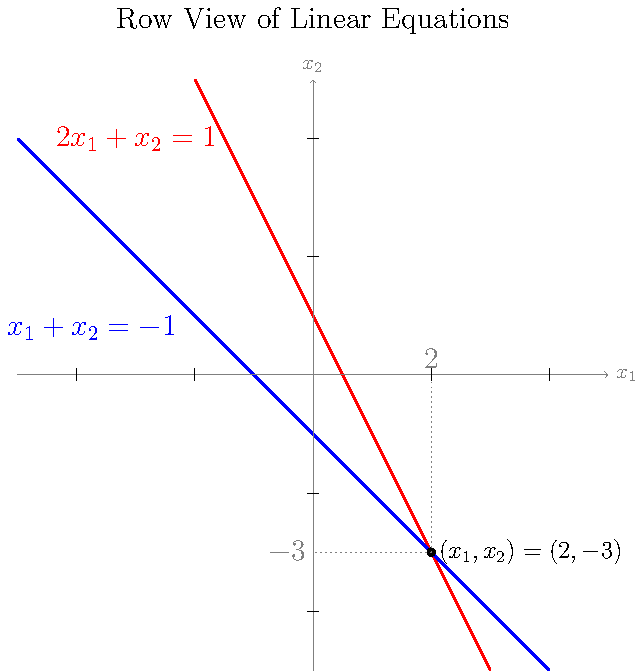
\includegraphics[width=0.5\textwidth]{figure/chapter03/lineqrowview.pdf}
    \caption{The row view of a system of two linear equations with two unknowns. The individual equations and lines are depicted in red and blue color in the plot. The intersection of these two lines is the solution to the problem, which is depicted by the black circle at $(2, -3)$.}
    \label{fig:ch03-lineq-row-view}
\end{figure}
The row view for a system of $n$ linear equations with $m$ unknowns is is a set of $n$ is depicted in $\mb{R}^m$, while the column view is depicted in $\mb{R}^n$. We will almost exclusively only make use of the column view for understanding linear equations and their solutions, as this view provides a more intuitive understanding than the row view. The row view is useful for when dealing with two unknowns, but becomes complicated for system of equations with more than two unknowns. 

We will now look at two types of applications where we come across linear equations: control problems and estimation problems. The equations have the same form in both cases, its our interpretation of ther different terms that changes.

\begin{figure}[h]
    \centering
    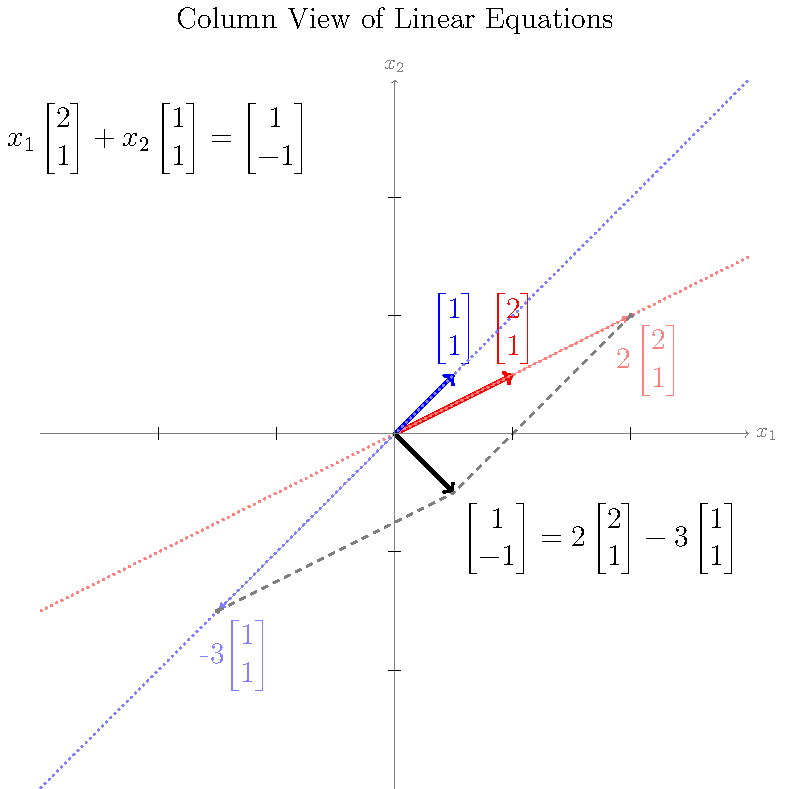
\includegraphics[width=0.714\textwidth]{figure/chapter03/lineqcolview.pdf}
    \caption{The set of all real numbers with magnitude $1$. This set contains two numbers $\lc -1, 1 \rc$.}
    \label{fig:ch03-lineq-col-view}
\end{figure}

\subsection{Linear equations in control problems}
Control problems are ones where the unknown $\mf{x}$ is the input to a system whose output is $\mf{b}$, and the matrix $\mf{A}$ is the system matrix mapping the inputs to the outputs. In control problems of the form $\mf{A}\mf{x} = \mf{b}$, the system matrix is known, and we wish to produce a desired output $\mf{b}$. We would like to find out the input $\mf{x}$ that produces the output for this system. The goal of solving $\mf{A}\mf{x} = \mf{b}$ in control problems, are to then apply these inputs to the real system to have it produce the output we desire. In such control problems, we ideally would like to have more inputs than outputs, which gives us more flexibility in controlling the system's output. This corresponds to system matrix is fat in this case ($n > m$); when $A$ is full rank, there are infinitely many inputs that produce the same output.

\begin{boxedstuff}
    \vspace{4mm}
    \noindent{\large \textbf{Examples of control problems}}
    \hrule
    \begin{example}
        \textbf{Radiotherapy}. Radiotheray or radiation therapy is a medical procedure where high-energy radiation is used to target and destroy cancer cells. Radiation therapy involves a radiation planning step, where the appropriate radiation dose is determined for delivery the desired dose to the cancers cells. The dose plannign step ca be formulated as a $\mf{A}\mf{x} = \mf{b}$ problem, where $\mf{A}$ is the radiation dose distribution matrix, $\mf{b}$ is the vector of desired radiation dose to the cancer cells, and $\mf{x}$ is the vector of unknown radiation dose to be delivered to the patient. We note that this descritpion is a simplification of the actual radiation therapy process. We will look at a more realistic description in Chapter~\ref{p04-chp:linprog} on Linear Programming.
    \end{example}
    \begin{example}
        \textbf{Robotics}: In robotics, we can control the motion and interaction of a robot by controlling the input to the actuators of the robot. Consider a robot with a serial, open kinematic chain consisting of $m$ joints (with one actuator per joint) which control the 3D position of its end-effector. The relationship between the joint angles and the end-effector position is non-linear. However, for a given joint configuration (i.e., a fixed set of values for the joint angles), the relationship between the joint velocities $\bm{\omega} \in \mb{R}^m$ and the end-point velocity $\mf{v} \in \mb{R}^3$ is linear, which are related through the robot's \textit{Jacobian} matrix $\mf{J} \in \mb{R}^{3 \times m}$.
        \[  \mf{v} = \mf{J} \bm{\omega} \]
        Given the desired end-effector velocity $\mf{v}\in \mb{R}^3$ for a given joint configuration (i.e., know Jacobian matrix $\mf{J} \in \mb{R}^{3 \times m}$), the control problem is to determine the unknown joint velocities $\bm{\omega} \in \mb{R}^m$ that will produce the desired end-effector velocity.
    \end{example}
\end{boxedstuff}


\subsection{Linear equations in estimation problems}
Estimation problems are ones where the unknown $\mf{x}$ is the set of parameter associated with a system that cannot be directly observed or measured, adn $\mf{b}$ is the of measureable quantities of the system, and the matrix $\mf{A}$ is the system matrix that determines how the parameters parameters influnce the system's measurable quantities. In estimation problems we are interested in solving $\mf{A}\mf{x} = \mf{b}$, because want to the know the internal parmeters $\mf{x}$ of the system that are responsible for generating the observed quantities $\mf{b}$. Note that unlike the control problems, we cannot modify that system parameters $\mf{x}$; in these problem solving for $\mf{x}$ is a way of knowing something about the system that we cannot directly observe. In these problems, the system matrix and measurements are known, and we ideally would like to have more measurements than the number of parameters associated with the system, as this allow redundancy in the measurements to account for noise in our measurements and obtain more accurate estimates of the system parameters. This corresponds to system matrix is tall in this case ($n > m$); when $A$ is full rank, then the outputs are forces to be constrained to lie in a smaller subspace of dimension $m$ in $\mb{R}^n$; these constrains are what help us beat noise when we have multiple measurements. We will discuss this in more detail in Chapter~\ref{p03-chp:statsest} on Statistical Estimation.

\begin{boxedstuff}
    \vspace{4mm}
    \noindent{\large \textbf{Examples of estimation problems}}
    \hrule
    \begin{example}
        \textbf{Computed tomography (CT)}.  CT is a medical imagining modality of creating cross-sectional images of the body using x-rays. X-ray passed through a cross-section of the body, and received by detectors on the other side. The internal distribution of the absoptivity of the body tissue is estimated from measurements made by shooting x-ray through the body from different angles. This can be fomulated as a $\mf{A}\mf{x} = \mf{b}$ problem, which is explained in a bit more details in the Exercises section of this chapter.
    \end{example}
    \begin{example}
        \textbf{System identification of linear dynamical systems}: The process of estimating the parameters of a linear dynamical system from records of its input and output data is referred to as \textit{system identification}. This discussed in detail in the Applications section (Section~\ref{sec:ch03-appln}) of this chapter.
        % Consider the following simple example of a discrete-time linear dynamical system,
        % \[ y_n = a y_{n-1} + b_0 u_n, \quad 0 \leq n < N \]
        % Let's assume that we have $N$ measurements of the input $x_n$ and output $y_n$ of the system. If we represent The goal of system identification is to estimate the unknown parameters $a$ and $b_0$ of the system. This can be formulated as a $\mf{A}\mf{x} = \mf{b}$ problem, where $\mf{A}$ is the system matrix, $\mf{x}$ is the vector of unknown parameters, and $\mf{b}$ is the vector of measurements. We will look at a more realistic description in Chapter~\ref{p03-chp:statsest} on Statistical Estimation.
    \end{example}
\end{boxedstuff}

\section{Solutions of linear equations}\label{sec:ch03-soln-lineq}
We will not look at the procedure for solving a system of linear equations, but rather understand the different possible solution(s) to a system of linear equations, and how the properties of the matrix $\mf{A}$ and the vector $\mf{b}$ determine the solution(s) of $\mf{A}\mf{x} = \mf{b}$. A system of linear equations can be one of the following three types: (a) unique solution, (b) infinitely many solution, and (c) no solution. We will now look at the conditions under which each of these types of solutions occur.

\subsection{Unique solution}
A unique solution is possible under two conditions:
\begin{itemize}
    \item \textbf{Square, full rank } $\mf{A} \in \mb{R}^{n \times n}$: When $\mf{A}$ is square and full rank, then the span of the columns of $\mf{A}$ is $\mb{R}^n$ and are linearly independent. This implies that the columns of $\mf{A}$ form a basis for $\mb{R}^n$. Thus, any vector in $\mb{R}^n$ can be represents as a linear combination of the columns of $\mf{A}$ and in a unique manner. Thus, there is a unique solution to the system of linear equations. 
    
    \item \textbf{Tall, full rank } $\mf{A} \in \mb{R}^{n \times m}$ and $\mf{b} \in \textbf{span}\lc \mf{a}_1, \mf{a}_2, \cdots \mf{a}_m\rc$: When a tall matrix $\mf{A}$ is full rank, then $\text{rank}\lp \mf{A} \rp = m$. The columns of $\mf{A}$ are linearly independent and span a subspace $\mc{S}$ of $\mb{R}^n$ of dimension $m$. The columns of $\mf{A}$ also form basis for the subspace $\mc{S}$. Thus, if $\mf{b}$ is in $\mc{S}$, then a unique linear combination of the columns of $\mf{A}$ would produce $\mf{b}$. But what happens when $\mf{b} \notin \mc{S}$, then what?
\end{itemize}

The geometry of the unique solution is depicted in Figure \hl{xxx}.

\subsection{Infinitely many solutions}

\subsection{No solution}


\section{Revisiting linear independence}

\section{Four fundamental subspaces of $\mf{A}$}


\section{Applications}\label{sec:ch03-appln}


\section{Exercise}
\vspace{-0.5cm}
\begin{center}
    \rule{\textwidth}{1pt}
\end{center}

\begin{enumerate}
    \item Derive force and displacement relationship for a series of $n+1$ springs (with spring constants $k_i$) connected in a line. There are $n$ nodes, with $f_i$ and $x_i$ representing the force applied and resulting displacement at the $i^{th}$ node. 
    \begin{center}
        \begin{tikzpicture}
            \fill [pattern = north east lines] (-0.15,-0.325) rectangle (0,0.325);
            \draw[thick] (0,-0.34) -- (0,0.34);
    
            \draw[thick] (0,0) -- (0.2,0);
            \draw[decoration={aspect=0.3, segment length=1mm, amplitude=1mm, coil,},decorate, thick] (0.2,0) -- (1.0,0);
            \draw[thick] (1.0,0) -- (1.2,0);
            \node[black] at (1.18,-0.02) {$\bullet$};
            \node[black] at (0.6,0.4) {$k_1$};
            \draw[dashed, thin] (1.18,0) -- (1.18,-0.75) node[below]{$x_1$};
            \draw[->,thick] (1.18,-0.4) -- (1.58,-0.4) node[below]{$f_1$};
    
            
            \draw[thick] (1.2,0) -- (1.4,0);
            \draw[decoration={aspect=0.3, segment length=1mm, amplitude=1mm, coil,},decorate, thick] (1.4,0) -- (2.2,0);
            \draw[thick] (2.2,0) -- (2.4,0);
            \node[black] at (2.38,-0.02) {$\bullet$};
            \node[black] at (1.8,0.4) {$k_2$};
            \draw[dashed, thin] (2.38,0) -- (2.38,-0.75) node[below]{$x_2$};
            \draw[->,thick] (2.38,-0.4) -- (2.88,-0.4) node[below]{$f_2$};
            
            \draw[thick] (2.4,0) -- (2.6,0);
            \draw[decoration={aspect=0.3, segment length=1mm, amplitude=1mm, coil,},decorate, thick] (2.6,0) -- (3.4,0);
            \draw[thick] (3.4,0) -- (3.6,0);
            \node[black] at (3.0,0.4) {$k_3$};
    
            \node[black] at (4.0, 0) {$\cdots$};
    
            \draw[thick] (4.2,0) -- (4.4,0);
            \draw[decoration={aspect=0.3, segment length=1mm, amplitude=1mm, coil,},decorate, thick] (4.4,0) -- (5.2,0);
            \draw[thick] (5.2,0) -- (5.4,0);
            \node[black] at (4.18,-0.02) {$\bullet$};
            \node[black] at (4.8,0.4) {$k_{n+1}$};
            \draw[dashed, thin] (4.18,0) -- (4.18,-0.75) node[below]{$x_n$};
            \draw[->,thick] (4.18,-0.4) -- (4.68,-0.4) node[below]{$f_n$};
    
            \fill [pattern = north east lines] (5.4,-0.325) rectangle (5.55,0.325);
            \draw[thick] (5.4,-0.34) -- (5.4,0.34);
        \end{tikzpicture}
    \end{center}
    \begin{enumerate}
        \item Represent the relationship in the following form, 
        \[ \mf{f} = \mf{Kx}; \,\,\, \mf{f} = \begin{bmatrix}f_1\\ f_2\\ \vdots\\ f_n\end{bmatrix}; \,\,\, \mf{x} = \begin{bmatrix}x_1 \\ x_2 \\ \vdots \\ x_n\end{bmatrix}\]
        \item What kind of a pattern does $\mf{K}$ have? 
        \item \textcolor{blue}{\textbf{[Programming]}} Consider a specific case where $n = 4$ and $k = 1.5 N.m^{-1}$. What should be forces applied at the four nodes in order to displace the spring $\mf{x} = \begin{bmatrix*} 0.5 \\ -0.5 \\ 0 \\ 0 \end{bmatrix*}m$. 
    \end{enumerate}
    
    \item Consider the following electrical circuit with rectangular grid of resistors $R$. The input to this grid is a set of current injected at the top node as shown in the figure, such that $\sum_{k=1}^5i_k = 0$.
    \vspace{-0.25cm}
    \begin{center}
    \begin{circuitikz}[scale=0.9]
        \draw (2,0) to[R,*-*] (0,0)
        to[R,*-*] (0,2) to[R,*-*] (0,4) to[R,*-*] (2,4)
        to[R,*-*] (2,2) to[R,*-*] (2,0) to[R,*-*] (4,0)
        to[R,*-*] (4,2) to[R,*-*] (4,4) to[R,*-*] (6,4)
        to[R,*-*] (6,2) to[R,*-*] (6,0) to[R,*-*] (8,0)
        to[R,*-*] (8,2) to[R,*-*] (8,4) to[R,*-*] (6,4);
    
        \draw (0,2) to[R,*-*] (2,2);
        \draw (2,4) to[R,*-*] (4,4);
        \draw (2,2) to[R,*-*] (4,2);
        \draw (4,2) to[R,*-*] (6,2);
        \draw (4,0) to[R,*-*] (6,0);
        \draw (6,2) to[R,*-*] (8,2);
    
        \draw (0,5) node[above]{$i_1$} to[short, o-] (0,4);
        \draw (2,5) node[above]{$i_2$} to[short, o-] (2,4);
        \draw (4,5) node[above]{$i_3$} to[short, o-] (4,4);
        \draw (6,5) node[above]{$i_4$} to[short, o-] (6,4);
        \draw (8,5) node[above]{$i_5$} to[short, o-] (8,4);
    \end{circuitikz}
    \end{center}
    
    Express the relationship between the voltages at the different nodes (represented by $\bullet$ in the figure) and the net current flowing in/out of the node in the following form, $\mf{G}\mf{v} = \mf{i}$. Where, $\mf{G}$ is the conductance matrix, $\mf{v}$ is the vector of node voltages, and $\mf{i}$ is the vector representing the net current flow in/out of the different node. 
    
    \item \textbf{Two point boundary problem.} $\mf{A}\mf{x} = \mf{b}$ is often encountered in many practical applications. One such application is the numerical solution of differential equations of the following form,
    \[ \sum_{i=0}^M a_{i}\ct{x}y^{\ct{i}}\ct{x} = f\ct{x} \]
    where, $x \in \dt{a, b}$ and $y\ct{a} = \alpha, y\ct{b} = \beta$. 
    
    Numerical methods are often employed for obtaining an approximate estimate of $y\ct{x}$ at discrete points in the interval $\dt{a,b}$. The interval is divided into subintervals of width $\Delta x$. The derivate of $y\ct{x}$ at the different nodes (points between two subintervals) can be approximated as the following,
    \begin{align}
    y'\ct{x_i} &= \frac{y\ct{x_i + \Delta x} - y\ct{x_i - \Delta x}}{\Delta x}\nonumber\\
    y''\ct{x_i} &= \frac{y\ct{x_i + \Delta x} + 2y\ct{x_i} - y\ct{x_i - \Delta x}}{\Delta x^2} \nonumber
    \end{align}
    where, $x_i = a + i\Delta x, \,\, 0 \leq i \leq N+1$, and $b - a = \ct{N+1} \Delta x$. Addition and subtracting the above two equations and neglecting terms involving higher orders of $\Delta x$, we get the following approximations for the derivatives of $y\ct{x}$ at $x_i$.
    
    Replacing the derivatives of $y\ct{x}$ by the above approximations and evaluating the equation at the different nodes $x_i$s, we arrive a set of $N$ linear equations with $N$ unknowns $y\ct{x_1}, y\ct{x_2}, \ldots y\ct{x_N}$. 
    
    Using this approach, compute an approximate solution for $y\ct{x}$ for the following differential equations over the interval $x \in \dt{0, 1}$.
    \begin{enumerate}
            \item $y''\ct{x} = -x$
            \item $y''\ct{x} + y'\ct{x} = x$
    \end{enumerate}
    \textcolor{blue}{\textbf{[Programming]}} Solve these equations for different values of $\Delta x$, and compare the resulting approximate solution for $y\ct{x}$ with the exact solution.   Present your results as a plot the solution $y\ct{x_i}$ versus $x_i$. 

    Comment on the dependence of the solution $\ct{x}$ on $\Delta x$. What is the best value for $\Delta x$ to use in solving these equations? 
    
    \item \textbf{Ill-conditioned systems.} A system $\mf{A}\mf{x} = \mf{b}$ is said to be ill-conditioned when small changes in the components of $\mf{A}$ or $\mf{b}$ can produce large changes in the solution $\mf{x}$. Consider the following system,
    \begin{align}
    x - y &= 100 \nonumber \\
    10 + \ct{9 + \Delta}y &= 0 \nonumber
    \end{align}
    \textcolor{blue}{\textbf{[Programming]}} Find the solutions of the system for different values of $\Delta = -2, -1, 0, 1, 2$. How do the solutions change with $\Delta$. 

    Now consider the following system,
    \begin{align}
    x - y &= 100 \nonumber \\
    10 - \ct{9 + \Delta}y &= 0 \nonumber
    \end{align}
    \textcolor{blue}{\textbf{[Programming]}} Find the solutions of the system for different values of $\Delta = -2, -1, 0, 1, 2$. How do the solutions change with $\Delta$. 
    
    The second system is an example of an ill-conditioned system. What can you say about the geometries of these two systems? 
    
    \item \textbf{Connectivity matrices.} Another common application of matrices is in graph theory. A graph is a set of vertices or nodes connected by edges, as show in the following figure. $A$-$F$ are the nodes of the graph, and the lines with the arrows are the edges that convey information about the connections or relationships between the nodes.
    \begin{center}
        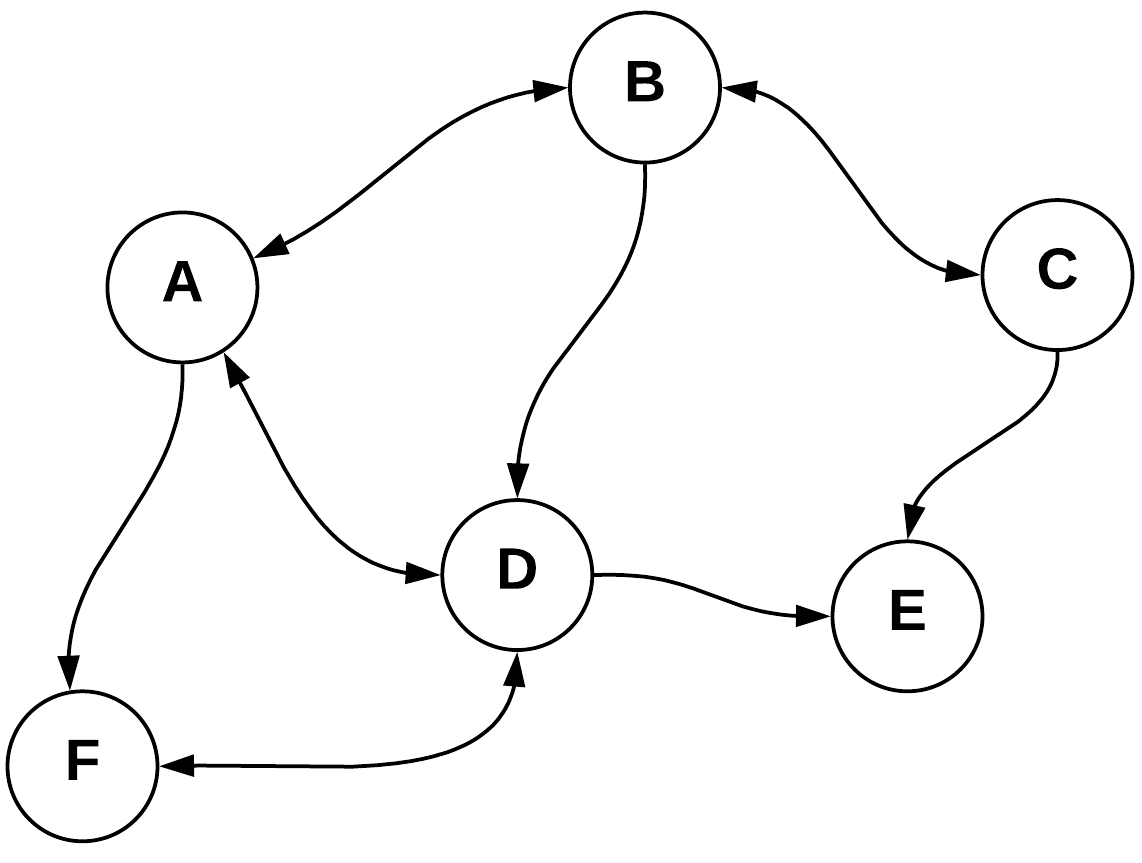
\includegraphics[width=0.5\columnwidth]{figure/chapter03/graph.png}
    \end{center}
    The above graph can be thought as a representation of different places in a city (represented by the nodes), and the lines with the arrows represent the roads connecting these different places. A line with two arrows allow two-way traffic, while line with single arrow only allow one way traffic. The connectivity between the different places can be summarized though the connectivity matrix $\mf{C} \in \mb{R}^{n \times n}$, where $n$ is the number of nodes in the graph. The elements of this connectivity matrix  represents whether or not there is a direct path between two places.
    \[ 
    c_{ij} = \begin{cases}
        1 & \text{there is a direct road between places } i \, \& \,j. \\
        0 & \text{otherwise.}
    \end{cases}
    \]
    The diagonal element of $\mf{C}$ are zero, $c_{ii} = 0$.
    
    Write down the connectivity matrix $\mf{C}$ for the graph shown above. How can we use the matrix $\mf{C}$ to answer the following questions? Explain exact matrix operation you would perform to answer these questions (Hint: Consider higher power of $\mf{C}$).
    \begin{enumerate}
        \item Is there a path between two places $i$ and $j$ that goes via one other place? For example, we can go from $A$ to $D$ via $B$.
        \item How many paths are there between places $i$ and $j$ that goes via three other places?
    \end{enumerate}
    
    \item \textbf{Computed Tomography} (CT) is a medical imaging technique that is used to reconstruct the internal structure of an object from a set of X-ray measurements. The object is placed between an X-ray source and a detector. The X-ray source and the detector are rotated around the object, and the X-ray measurements are recorded at different angles. The X-ray measurements are then used to reconstruct the internal structure of the object.
    \begin{figure}[h]
        \centering
        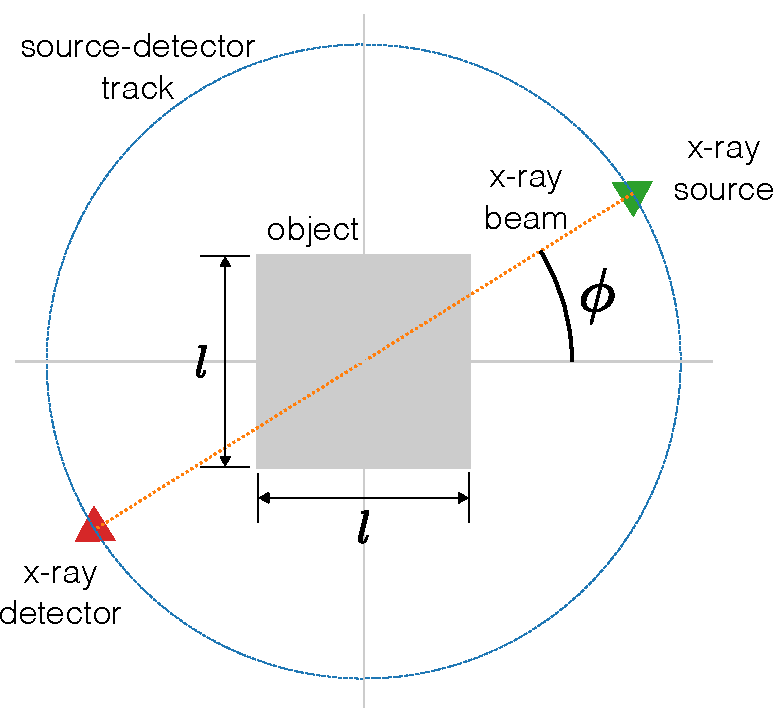
\includegraphics[width = 0.6\textwidth]{figure/chapter03/ct_setup_full.pdf}
        \caption{A simplified CT set-up with a single X-ray source and a single detector, that are located diametrically opposite to each other and can rotate to any scan angle $\phi$. The object is placed between the X-ray source and the detector, which is depicted by the gray square of side $l$. The x-ray originates from the green triangle (x-ray source), passes through the object, and is detected by the red triangle (detector). The x-ray undergoes attenuation as it passes through the object. Different points in the objects are most likely to have different attentuation coefficients, and the goal of CT is toe reconstruct of spatial map of the attentuation within the object, which provides a measure of the internal structure of the object.}
        \label{fig:ct}
    \end{figure}
    
    The x-ray attentuation equation is given by,
    \[ I_o = I_i \exp\lp -\mu l \rp \]
    where, $I_i$ is the intensity of the x-ray entering an object with fixed attentuation coefficient $\mu$, $I_o$ is the intensity of the x-ray existing the object, and $l$ is the path length of the x-ray in the object. 
    
    In general, the attenuation coefficient is a function of the position within the object, $\mu = \mu\ct{x,y}$. The goal of CT is to reconstruct the spatial map of the attenuation coefficient $\mu\ct{x,y}$.
    
    Let $L$ represent the line segment of the x-ray within the object as shown in Figure~\ref{fig:ct}, and the attentuation outside the object is assumed to be zero. If $I_s$ is the intensity of the x-ray leaving the source, the intensity of the x-ray reaching the detector $I_d$ is given by,
    \[ I_d = I_s \exp\lp - \int_L \mu \ct{x, y} dl \rp \]
    where, $dl$ is the differential length along the line segment $L$, which is a function of $x, y$. The integral in the above equation is the line integral of the attenuation coefficient $\mu\ct{x,y}$ along the line segment $L$.
    
    We wish to solve this problem using a computer by posing it as a set of linear equations relating the attenuation coefficient $\mu\ct{x,y}$ to the x-ray intensity measurements $I_d$. For simplicity, we will assume $I_s = 1$. First, we simplify the above integration equation by taking the log on both sides, which results in,
    \[ \ln I_d = - \int_L \mu \ct{x, y} dl \]
    Explain the why above step is valid. Do we need to worry about the case where $I_d = 0$? 
    
    Discretize the object into $n \times n$ grid of pixels, and assume that attentuation coefficient within each pixel to be constant. For any given scan angle $\phi$ you need to find out the pixels the line segment $L$ passes through, along with the path length of the x-ray line segment within each pixel. Derive the discrete expression relating the x-ray intensity measurements $I_d$ to the attenuation coefficient $\mu\ct{x,y}$ for a given scan angle $\phi$, assuming a discretized object $n \times n$. Write down the above expression in the following form 
    \[ \tilde{\mf{a}}\ct{\phi}^\top \mf{x} = y\ct{\phi} \]
    where, $\mf{x} \in \mb{R}^{n^2}$ is the vector of unknown attenuation coefficients of the pixels in the image, $\tilde{\mf{a}}\ct{\phi} \in \mb{R}^{n^2}$ is the vector relating the attentuation coefficients to the detector measurement for the given source-detector angle $\phi$ and $y\ct{\phi} \in \mb{R}$ is the log of the x-ray intensity measured by the detector. 
    
    If we make a set of such measurements for $m$ different angles $\phi_1, \phi_2, \cdots \phi_m$, we can write the above equation in the following matrix form,
    \[ \mf{A}\mf{x} = \mf{y} \]
    \[ \mf{A} = \bmxc \tilde{\mf{a}}_1 & \tilde{\mf{a}}_2 & \cdots & \tilde{\mf{a}}_m\emx^\top \in \mb{R}^{m \times n^2}\quad \mf{y} = \bmxc y_1 & y_2 & \cdots & y_m\emx^\top \in \mb{R}^{m} \]
    where, $\tilde{\mf{a}}_i$ is the vector relating the attentuation coefficients to the detector measurement for the source-detector angle $\phi_i$ and $y_i$ is the log of the x-ray intensity measured by the detector for the angle $\phi_i$.
    
    \textbf{Forward problem for CT}. Once you've derived the above matrix linear equation, we can use it to simulate a CT scan by computing $\mf{y}$ for a given $\mf{x}$ and scan angle $\phi$, we can compute intensity of the x-ray that will be measured by the detector. Consider the following three objects that we wish to scan using out CT scanner. Given the relatively simple geometry of the spatial distribution of the attenuation coefficients $\mu\ct{x,y}$, you can use the $\mf{A}\mf{x} = \mf{y}$ equation to solve the forward CT problem, i.e., compute the detector output for different scan angles for the given object. For the three objects below, come up with a pixelation scheme for the objects ($n$ number of pixels and pixel dimensions) and come up with the matrix $\mf{A}$ for the three objects. Use this matrix $A$ and the known pixel attentualtion coefficients $\mf{x}$ to compute the detector outputs for 360 scan angle $\phi = 0\deg, 1\deg, 2\deg, \ldots 359\deg$. Assume $l = 1 unit$.
    
    \textcolor{blue}{\textbf{[Programming]}} Write a python program to compute and plot the detector output for the different scan angles.
    
    \textbf{Suggestion:} \textit{For each object write a function that will take in the scan angle, the object side length $l$, and return the row vector $\tilde{\mf{a}}\ct{\phi}^\top$. Use this function to compute the matrix $\mf{A}$ for the three objects.}
    
    \begin{figure}[h]
        \centering
        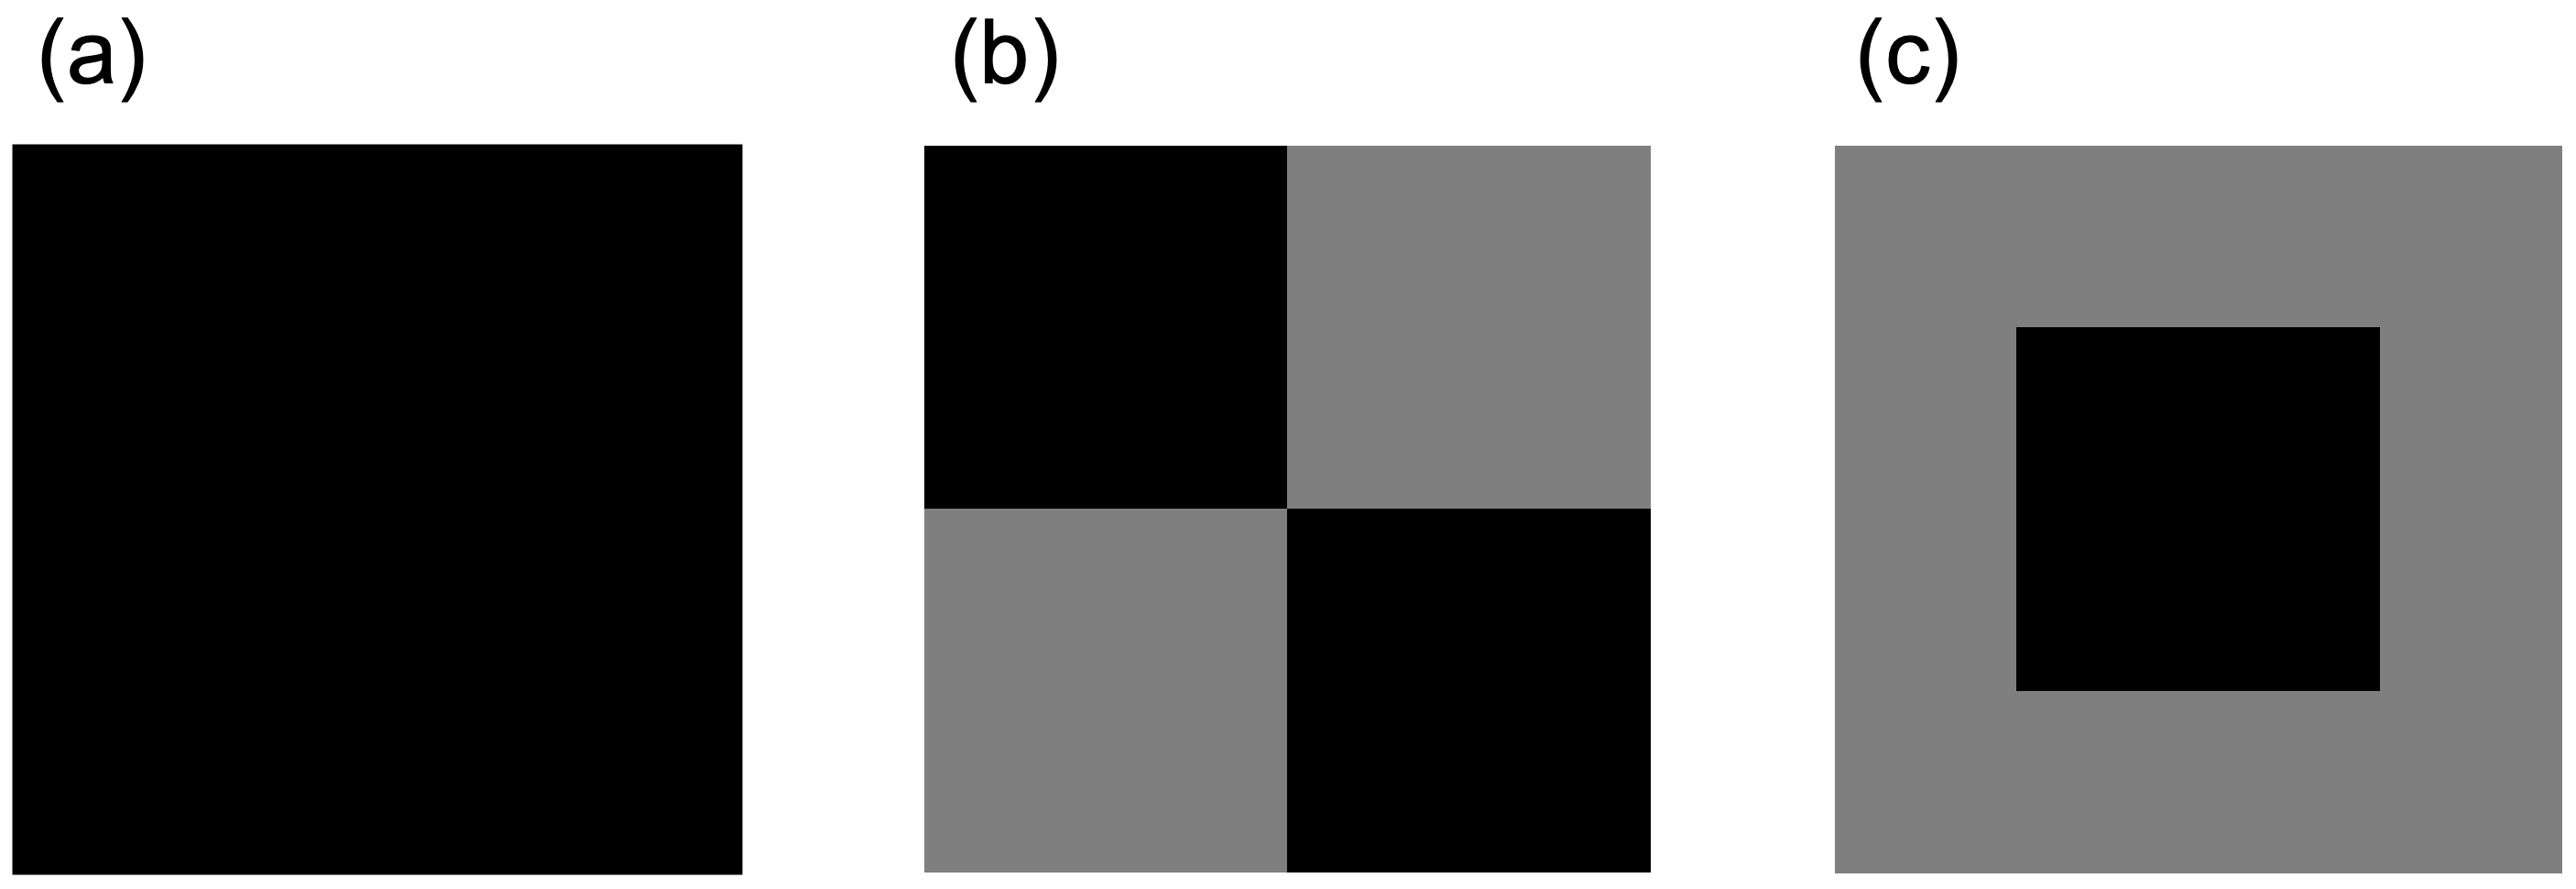
\includegraphics[width = 0.8\textwidth]{figure/chapter03/ct_images.png}
        \caption{Three objects that are to be scanned using the CT scanner described in the figure above. The black regions in this image represent the pixels with attenuation coefficient $\mu = 1$, and the gray regions represent the pixels with attenuation coefficient $\mu = 0.5$.}
        \label{fig:ctimages}
    \end{figure}
\end{enumerate}
    